% !TEX root = ../thesis.tex

\chapter{\name{Eliashberg} theory}

Based on the results presented in the previous chapter, one can formulate a set
of equations, namely the \name{Eliashberg} equations, which determine
self-energies for both normal and anomalous \name{Green} functions, the latter
being suitable order parameters for the superconducting state.

To that end it is convenient to combine the \name{Green} functions of interest
into a $2 \times 2$ matrix, i.e. to use the \name{Nambu} formalism, which is
presented in the first section. With that, the general form of the
\name{Eliashberg} equations on the imaginary frequency axis are derived,
followed by some common simplifications which assume (i) a $\vec k$-independent
self-energy, (ii) a constant density of states and (iii) the suitability of a
\name{Coulomb} pseudo-potential. Next, it is shown how the results, which are
generally just the numerical values corresponding to a finite set of
\name{Matsubara} frequencies rather than analytical expressions, can be
continued to the real axis by means of \name{Padé} approximants. Finally, it is
outlined how \name{McMillan} and \name{Dynes}' formula for the critical
temperature can be obtained from the \name{Eliashberg} theory.

\section{\name{Nambu} formalism}

As found by \name{Nambu} \cite{Nambu60}, the \text{Dyson} equations for all four
electronic \name{Green} functions introduced at the beginning of
Section~\ref{Model interactions} can be compactly formulated as a single matrix
equation:
%
\begin{equation*}
    % !TEX root = ../thesis.tex
%
\tikzsetnextfilename{nambu-dyson}
%
\begin{tikzpicture}[yscale=-1]
    \foreach \r in {
        (-0.25, 0.25), (2.25, 0.25), (4.75, 0.25), (7.00, 0.25), (9.25, 0.25),
        ( 2.25, 1.50), (2.25, 2.75)}
        \node at \r {$\Bigg[$};

    \foreach \r in {
        ( 1.75, 0.25), (4.25, 0.25), (6.75, 0.25), (9.00, 0.25), (11.25, 0.25),
        (12.25, 1.50), (8.25, 2.75)}
        \node at \r {$\Bigg]$};

    \foreach \r in {
        (2.5, 0.00), (5.0, 0.00), ( 2.5, 1.25), (3.5, 1.25),
        (5.5, 1.25), (8.5, 1.25), (10.5, 1.25), (2.5, 2.50),
        (3.5, 2.50), (4.5, 2.50), ( 6.5, 2.50), (4.5, 3.00)}
        \draw [backward] \r -- +(0.5, 0);

    \foreach \r in {(3.75, 0), (6.25, 0), (2.75, 0.5), (5.25, 0.5)}
        \node at \r {$0$};

    \foreach \r in {
        (3.5, 0.50), (6.0, 0.50), ( 3.5, 1.75), (5.5, 1.75),
        (7.5, 1.75), (8.5, 1.75), (10.5, 1.75), (7.5, 2.50),
        (3.5, 3.00), (5.5, 3.00), ( 6.5, 3.00), (7.5, 3.00)}
        \draw [forward] \r -- +(0.5, 0);

    \draw [backward] (4, 2.5) arc (180:360:2.5mm);
    \draw [ outward] (7, 2.5) arc (180:360:2.5mm);
    \draw [  inward] (4, 3.0) arc (180:360:2.5mm);
    \draw [ forward] (7, 3.0) arc (180:360:2.5mm);

    \foreach \r in {(4, 2.5), (7, 2.5), (4, 3), (7, 3)}
        \draw [phonon] \r -- +(0.5, 0);

    \foreach \r in {(0, 0.0), ( 9.5, 0.0), ( 4.5, 1.25), ( 4.5, 1.75)}
        \draw [backward, double] \r -- +(0.5, 0);
    \foreach \r in {(1, 0.0), (10.5, 0.0), ( 9.5, 1.25), ( 9.5, 1.75)}
        \draw [ outward, double] \r -- +(0.5, 0);
    \foreach \r in {(0, 0.5), ( 9.5, 0.5), ( 6.5, 1.25), ( 6.5, 1.75)}
        \draw [  inward, double] \r -- +(0.5, 0);
    \foreach \r in {(1, 0.5), (10.5, 0.5), (11.5, 1.25), (11.5, 1.75)}
        \draw [ forward, double] \r -- +(0.5, 0);

    \foreach \r in {(7.25, 0.0), (4, 1.25), ( 9, 1.25)}
        \draw [backward, double] \r arc (180:360:2.5mm);
    \foreach \r in {(8.25, 0.0), (6, 1.25), (11, 1.25)}
        \draw [ outward, double] \r arc (180:360:2.5mm);
    \foreach \r in {(7.25, 0.5), (4, 1.75), ( 9, 1.75)}
        \draw [  inward, double] \r arc (180:360:2.5mm);
    \foreach \r in {(8.25, 0.5), (6, 1.75), (11, 1.75)}
        \draw [ forward, double] \r arc (180:360:2.5mm);

    \foreach \r in {
        (7.25, 0), (8.25, 0), (7.25, 0.5), (8.25, 0.5),
        (4, 1.25), (6, 1.25), (9, 1.25), (11, 1.25),
        (4, 1.75), (6, 1.75), (9, 1.75), (11, 1.75)}
        \draw [phonon, double] \r -- +(0.5, 0);

    \foreach \r in {
        (7.25, 0), (8.25, 0), (7.25, 0.5), (8.25, 0.5),
        (4, 1.25), (6, 1.25), (9, 1.25), (11, 1.25),
        (4, 1.75), (6, 1.75), (9, 1.75), (11, 1.75),
        (4, 2.50), (7, 2.50), (4, 3.00), ( 7, 3.00)}
        \fill \r circle (1.5pt) +(0.5, 0) circle (1.5pt);

    \foreach \r in {(2, 0.25), (2, 1.5)} \node at \r {$=$};

    \node at (2, 2.75) {$\approx$};

    \foreach \r in {
        (4.50, 0.25),
        (3.25, 1.25), (5.25, 1.25), (8.25, 1.75), (10.25, 1.25),
        (3.25, 2.50), (5.25, 1.75), (6.25, 3.00), (10.25, 1.75)}
        \node at \r {$+$};
\end{tikzpicture}%

\end{equation*}
%
or formally, where quantum numbers and frequency arguments are suppressed,
%
\begin{equation} \label{Nambu-Dyson equation}
    \begin{split}
        \begin{bmatrix}
            G & F \\
            \widetilde F & \widetilde G
        \end{bmatrix}
        &=
        \begin{bmatrix}
            G_0 & 0 \\
            0 & \widetilde G_0
        \end{bmatrix}
        +
        \begin{bmatrix}
            G_0 & 0 \\
            0 & \widetilde G_0
        \end{bmatrix}
        \begin{bmatrix}
            \Sigma^G & \Sigma^F \\
            \Sigma^{\widetilde F} & \Sigma^{\widetilde G}
        \end{bmatrix}
        \begin{bmatrix}
            G & F \\
            \widetilde F & \widetilde G
        \end{bmatrix}
        \\
        &=
        \begin{bmatrix*}[r]
            G_0 + G_0 \Sigma^G G + G_0 \Sigma^F \widetilde F
            & G_0 \Sigma^G F + G_0 \Sigma^F \widetilde G \\
            \widetilde G_0 \Sigma^{\widetilde F} G
            + \widetilde G_0 \Sigma^{\widetilde G} \widetilde F
            & \widetilde G_0 + \widetilde G_0 \Sigma^{\widetilde F} F
            + \widetilde G_0 \Sigma^{\widetilde G} \widetilde G
        \end{bmatrix*}
        \\
        &\approx
        \begin{bmatrix*}[r]
            G_0 + G_0 \Sigma^G_0 G_0 & G_0 \Sigma^F_0 \widetilde G_0 \\
            \widetilde G_0 \Sigma^{\widetilde F}_0 G_0 & \widetilde G_0
            + \widetilde G_0 \Sigma^{\widetilde G}_0 \widetilde G_0
        \end{bmatrix*}.
    \end{split}
\end{equation}

\tikz [baseline=-0.5ex] \draw [ inward] (0, 0) -- (0.5, 0); and
\tikz [baseline=-0.5ex] \draw [outward] (0, 0) -- (0.5, 0);
%
vanish, so does each term of the perturbation series of
%
\tikz [baseline=-0.5ex] \draw [ inward, double] (0, 0) -- (0.5, 0); and
\tikz [baseline=-0.5ex] \draw [outward, double] (0, 0) -- (0.5, 0);.
%
A non-zero self-consistent solution of the above integral equations may still
exist \cite[before Eq.~2.14]{Nambu60}.

Giving names to the involved matrices, the \name{Dyson} equation may be written
as $\vec G = \vec G_0 + \vec G_0 \vec \Sigma \vec G$ or even $\vec G^{-1} = \vec
G_0^{-1} - \vec \Sigma$, using inverse matrices. With the help of the
two-component operators
%
\begin{equation*}
    \vec \uppsi_{\vec k} =
    \begin{bmatrix}
        \op c_{\vec k \uparrow} \\
        \op c_{-\vec k \downarrow}^+
    \end{bmatrix}
    \quad \text{and} \quad
    \vec \uppsi_{\vec k}^+ =
    \begin{bmatrix}
        \op a_{\vec k \uparrow}^+ &
        \op a_{-\vec k \downarrow},
    \end{bmatrix}
\end{equation*}
%
the dressed (bare) \name{Green} function matrix is concisely defined as
%
\begin{equation*}
    \vec G_{\vec k}^{(0)}(\I \omega_n) = -\int \from 0 \till \beta \D \tau \,
    \E^{\I \omega_n \tau} \av{ \op U \,
    \vec \uppsi_{\vec k}(\tau) \,
    \vec \uppsi_{\vec k}^+(0)}_{(0)},
\end{equation*}
%
where $\op U = 1 + \op P + \op P^+$ ensures terms conserving the particle number
in all components \cite{ScalapinoSchriefferWilkins66}.

Introducing unit and \name{Pauli} matrices
%
\begin{equation*}
    \vec \sigma_0 =
    \begin{bmatrix}
        1 & 0 \\
        0 & 1
    \end{bmatrix},
    \quad
    \vec \sigma_1 =
    \begin{bmatrix}
        0 & 1 \\
        1 & 0
    \end{bmatrix},
    \quad
    \vec \sigma_2 =
    \begin{bmatrix}
        0 & -\I \\
        \I & 0
    \end{bmatrix},
    \quad
    \vec \sigma_3 =
    \begin{bmatrix}
    1 & 0 \\
    0 & -1
    \end{bmatrix}
\end{equation*}
%
and the real scalar functions $Z_{\vec k}(\I \omega_n)$, $\phi^{(\prime)}_{\vec
k}(\I \omega_n)$ and $\chi_{\vec k}(\I \omega_n)$, the self-energy matrix is
written as
%
\begin{align} \label{self-energy matrix}
    \vec \Sigma_{\vec k}(\I \omega_n) &= \I \omega_n
    [1 - Z_{\vec k}(\I \omega_n)] \vec \sigma_0
    + \phi _{\vec k}(\I \omega_n) \vec \sigma_1
    + \phi'_{\vec k}(\I \omega_n) \vec \sigma_2
    + \chi _{\vec k}(\I \omega_n) \vec \sigma_3
    \\ \notag
    &=
    \begin{bmatrix}
        \I \omega_n [1 - Z_{\vec k}(\I \omega_n)] + \chi_{\vec k}(\I \omega_n) &
        \phi_{\vec k}(\I \omega_n) - \I \phi'_{\vec k}(\I \omega_n) \\
        \phi_{\vec k}(\I \omega_n) + \I \phi'_{\vec k}(\I \omega_n) &
        \I \omega_n [1 - Z_{\vec k}(\I \omega_n)] - \chi_{\vec k}(\I \omega_n)
    \end{bmatrix},
\end{align}
%
With $[\vec G^0_{\vec k}(\I \omega_n)]^{-1} = \I \omega_n \vec \sigma_0 -
\epsilon_{\vec k} \vec \sigma_3$ the \textsc{Dyson} equation reads
%
\begin{align*}
    \vec G_{\vec k}^{-1}(\I \omega_n) &=
    [\vec G^0_{\vec k}(\I \omega_n)]^{-1} - \vec \Sigma_{\vec k}(\I \omega_n)
    \\
    &= \I \omega_n Z_{\vec k}(\I \omega_n) \vec \sigma_0
    - \phi _{\vec k}(\I \omega_n) \vec \sigma_1
    - \phi'_{\vec k}(\I \omega_n) \vec \sigma_2
    - [\epsilon_{\vec k} + \chi_{\vec k}(\I \omega_n)] \vec \sigma_3 \\
    &= \begin{bmatrix}
        \I \omega_n Z_{\vec k}(\I \omega_n)
        - \epsilon_{\vec k} - \chi_{\vec k}(\I \omega_n) &
        -\phi_{\vec k}(\I \omega_n) + \I \phi'_{\vec k}(\I \omega_n) \\
        -\phi_{\vec k}(\I \omega_n) - \I \phi'_{\vec k}(\I \omega_n) &
        \I \omega_n Z_{\vec k}(\I \omega_n)
        + \epsilon_{\vec k} + \chi_{\vec k}(\I \omega_n)
    \end{bmatrix},
\end{align*}
%
Inversion yields
%
\begin{align*}
    \vec G_{\vec k}(\I \omega_n) &= -\Theta_{\vec k}^{-1}(\I \omega_n) \{
        \I \omega_n Z_{\vec k}(\I \omega_n) \vec \sigma_0
        + \phi _{\vec k}(\I \omega_n) \vec \sigma_1
        + \phi'_{\vec k}(\I \omega_n) \vec \sigma_2
        + [\epsilon_{\vec k} + \chi_{\vec k}(\I \omega_n)] \vec \sigma_3 \}
    \\
    &= -\frac 1 {\Theta_{\vec k}(\I \omega_n)}
    \begin{bmatrix}
        \I \omega_n Z_{\vec k}(\I \omega_n)
        + \epsilon_{\vec k} + \chi_{\vec k}(\I \omega_n) &
        \phi_{\vec k}(\I \omega_n) - \I \phi'_{\vec k}(\I \omega_n) \\
        \phi_{\vec k}(\I \omega_n) + \I \phi'_{\vec k}(\I \omega_n) &
        \I \omega_n Z_{\vec k}(\I \omega_n)
        - \epsilon_{\vec k} - \chi_{\vec k}(\I \omega_n)
    \end{bmatrix},
\end{align*}
%
where the denominator is given by
%
\begin{equation*}
    \Theta_{\vec k}(\I \omega_n) = -\det \vec G_{\vec k}^{-1}(\I \omega_n)
    = [\omega_n Z_{\vec k}(\I \omega_n)]^2
    + [\epsilon_{\vec k} + \chi_{\vec k}(\I \omega_n)]^2
    + \phi ^2_{\vec k}(\I \omega_n)
    + \phi'^2_{\vec k}(\I \omega_n).
\end{equation*}
%
The excitation energies are the poles of $\vec G_{\vec k}(\I \omega_n)$, i.e.
the zeros of $\Theta_{\vec k}(\I \omega_n)$, which satisfy
%
\begin{align*}
    (\I \omega_n)^2 = \left[ \frac
        {\epsilon_{\vec k} + \chi_{\vec k}(\I \omega_n)}
        {Z_{\vec k}(\I \omega_n)}
    \right]^2
    + \frac
        {\phi_{\vec k}^2(\I \omega_n) + \phi'^2_{\vec k}(\I \omega_n)}
        {Z_{\vec k}^2(\I \omega_n)}
    \equiv \widetilde \epsilon^2_{\vec k}(\I \omega_n)
    + |\Delta_{\vec k}(\I \omega)|^2.
\end{align*}
%
This identifies $Z_{\vec k}(\I \omega_n)$ as a renormalization function,
$\chi_{\vec k}(\I \omega_n)$ as an energy shift and $\phi^{(\prime)}_{\vec k}(\I
\omega_n)$ as a suitable order parameter, since the energy gap of the
superconducting state turns out to be
%
\begin{align*}
    \Delta_{\vec k}(\I \omega) = \frac
        {\phi_{\vec k}(\I \omega_n) - \I \phi'_{\vec k}(\I \omega_n)}
        {Z_{\vec k}(\I \omega_n)}.
\end{align*}

\newpage

\section{General equations}

A comparison with the results derived in Section~\ref{Hubbard model}
(\ref{Holstein model}) reveals that the approximation made in
Eq.~\ref{Nambu-Dyson equation} is correct up to the first (second) order of the
perturbation series for the \name{Hubbard} (\name{Holstein}) model.
Consequently, for the \emph{\name{Hubbard-Holstein} model} one has
%
\begin{equation*}
    \vec \Sigma_{\vec k} (\I \omega_n)
    = \vec \Sigma_{\vec k} \super{el.}
    + \vec \Sigma_{\vec k} \super{ph.} (\I \omega_n).
\end{equation*}

The electronic part within the HF approximation according to Eq.~\ref{HF
approximation} reads
%
\begin{align*}
    \vec \Sigma_{\vec k} \super{el.} (\I \omega_n)
    = \frac{U}{N \beta} &\sum_{\vec q m}
        \vec G_{\vec q} \super{od.} (\I \omega_m)
    \\
    = -\frac{U}{N \beta} &\sum_{\vec q m} \frac
        { \phi _{\vec q}(\I \omega_m) \vec \sigma_1
        + \phi'_{\vec q}(\I \omega_m) \vec \sigma_2 }
        {\Theta_{\vec q}(\I \omega_m)},
\end{align*}
%
where \q{od.} indicates that the components which are not \q{off-diagonal} have
been nullified.

The corresponding phononic part is
%
\begin{multline*}
    \vec \Sigma_{\vec k} \super{ph.} (\I \omega_n)
    = -\frac{g^2}{N \beta} \sum_{\vec q m}
    \vec \sigma_3 \, \vec G_{\vec q}(\I \omega_m) \, \vec \sigma_3 \,
    D^0_{\vec k - \vec q}(\I \omega_n - \I \omega_m),
    \\
    = \frac{g^2}{N \beta} \sum_{\vec q m}
    \frac { \I \omega_m
              Z_{\vec q}(\I \omega_m) \vec \sigma_0
        - \phi _{\vec q}(\I \omega_m) \vec \sigma_1
        - \phi'_{\vec q}(\I \omega_m) \vec \sigma_2
        + [\epsilon_{\vec q} + \chi_{\vec q}(\I \omega_m)] \vec \sigma_3 }
        {\Theta_{\vec q}(\I \omega_m)}
    D^0_{\vec k - \vec q}(\I \omega_n - \I \omega_m),
\end{multline*}
%
where the \name{Pauli} matrices in the first line swap the sign of the
off-diagonal components.

From now on, $T = \beta^{-1}$ is used rather than $\beta$. A coefficient
comparison with Eq.~\ref{self-energy matrix} yields the
\emph{\textsc{Eliashberg} equations} for the \name{Hubbard-Holstein} model:
%
\begin{subequations} \label{Eliashberg equations}
    \begin{align}
        \I \omega_n [1 - Z_{\vec k}(\I \omega_n)] &= \frac T N
        \sum_{\vec q m} \frac
            {\I \omega_m Z_{\vec q}(\I \omega_m)}
            {\Theta_{\vec q}(\I \omega_m)}
        g^2 D^0_{\vec k - \vec q}(\I \omega_n - \I \omega_m),
        \\
        \phi^{(\prime)}_{\vec k}(\I \omega_n) &= -\frac T N
        \sum_{\vec q m} \frac
            {\phi^{(\prime)}_{\vec q}(\I \omega_m)}
            {\Theta_{\vec q}(\I \omega_m)}
        \big[ g^2 D^0_{\vec k - \vec q}(\I \omega_n - \I \omega_m) + U \big],
        \\
        \chi_{\vec k}(\I \omega_n) &= \frac T N
        \sum_{\vec q m} \frac
            {\epsilon_{\vec q} + \chi_{\vec q}(\I \omega_m)}
            {\Theta_{\vec q}(\I \omega_m)}
        g^2 D^0_{\vec k - \vec q}(\I \omega_n - \I \omega_m).
    \end{align}
\end{subequations}
%
$\phi_{\vec k}(\I \omega_n)$ and $\phi'_{\vec k}(\I \omega_n)$ obey equal
equations, leaving the phase of $\phi_{\vec k}(\I \omega) - \I \phi'_{\vec k}(\I
\omega_n)$ undetermined. This gauge invariance allows to assume $\phi'_{\vec
k}(\I \omega_n) = 0$ \cites[37]{AllenMitrovic82}[around Eq.~2.20]{Nambu60}.

Using the definitions \cite{MargineGiustino13}
%
\begin{align*}
    \mu = n(0) \, U,
        \quad
    \lambda_{\vec q}(\I \Omega_n) = -n(0) \, g^2 D_{\vec q}^0(\I \Omega_n),
        \quad
    n(\epsilon) = \frac{N(\epsilon)} N,
        \quad
    N(\epsilon) = \sum_{\vec k} \delta(\epsilon - \epsilon_{\vec k}),
\end{align*}
%
where $n(\epsilon)$ is the density of states per spin and unit cell, one can
equivalently write
%
\begin{multline*}
    \vec \Sigma_{\vec k} (\I \omega_n)
    = \frac T {N(0)} \sum_{\vec q m}
    \Theta_{\vec q}^{-1}(\I \omega_m) \big \{ \dots
        \\
        \dots \{
            - \I \omega_m Z_{\vec q}(\I \omega_m) \vec \sigma_0
            + \phi_{\vec q}(\I \omega_m) \vec \sigma_1
            - [\epsilon_{\vec q} + \chi_{\vec q}(\I \omega_m)] \vec \sigma_3
            \}
        \lambda_{\vec k - \vec q}(\I \omega_n - \I \omega_m)
        - \phi_{\vec q}(\I \omega_m) \vec \sigma_1 \mu
    \big \},
\end{multline*}
%
which yields a more common formulation of the \name{Eliashberg} equations:
%
\begin{subequations}
    \begin{align}
        Z_{\vec k}(\I \omega_n) &= 1 + \frac T {N(0)} \frac 1 {\omega_n}
        \sum_{\vec q m} \frac
            {\omega_m Z_{\vec q}(\I \omega_m)}
            {\Theta_{\vec q}(\I \omega_m)}
        \lambda_{\vec k - \vec q}(\I \omega_n - \I \omega_m),
        \\
        \phi_{\vec k}(\I \omega_n) &= \frac T {N(0)}
        \sum_{\vec q m} \frac
            {\phi_{\vec q}(\I \omega_m)}
            {\Theta_{\vec q}(\I \omega_m)}
        \big[ \lambda_{\vec k - \vec q}(\I \omega_n - \I \omega_m) - \mu \big],
        \\
        \chi_{\vec k}(\I \omega_n) &= -\frac T {N(0)}
        \sum_{\vec q m} \frac
            {\epsilon_{\vec q} + \chi_{\vec q}(\I \omega_m)}
            {\Theta_{\vec q}(\I \omega_m)}
        \lambda_{\vec k - \vec q}(\I \omega_n - \I \omega_m).
    \end{align}
\end{subequations}

\section{Local self-energy}

Assuming that the phonon part of the unperturbed \name{Hamilton} operator reads
%
\begin{equation*}
    \op H_0 \super{ph.}
    = \omega \sub E \sum_{\vec R} \op b_{\vec R}^+ \op b_{\vec R}
    = \omega \sub E \sum_{\vec q \vec q'} \frac 1 N \sum_{\vec R}
        \E^{\I (\vec q' - \vec q) \vec R} \op b_{\vec q'}^+ \op b_{\vec q}
    = \omega \sub E \sum_{\vec q} \op b_{\vec q}^+ \op b_{\vec q},
\end{equation*}
%
with a single Einstein frequency $\omega \sub E$, which is already renormalized,
one finds
%
\begin{align*}
    D_0(\I \Omega_n) &= -\int \from 0 \till \infty \D \omega \,
        \frac{2 \omega \, B(\omega)}{\Omega_n^2 + \omega^2}
    = -\frac{2 \omega \sub E}{\Omega_n^2 + \omega^2 \sub E}
    \quad \text{with} \quad
    B(\omega) = \delta(\omega - \omega \sub E) - \delta(\omega + \omega \sub E),
    \\
    \lambda(\I \Omega_n) &= \int \from 0 \till \infty \D \omega \,
        \frac{2 \omega \, \alpha^2 F(\omega)}{\Omega_n^2 + \omega^2}
    = \frac{2 \omega \sub E \, n(0) \, g^2}{\Omega_n^2 + \omega^2 \sub E}
    \quad \text{with} \quad
    \alpha^2 F(\omega) = n(0) \, g^2 B(\omega)
\end{align*}
%
independent of $\vec k$, i.e. \emph{local}. $B(\omega)$ and $\alpha^2 F(\omega)$
are \emph{phonon} and \emph{electron-phonon spectral functions}, respectively.
As a consequence, the same applies to the self-energy $\vec \Sigma$ and its
components $Z$, $\phi$ and $\chi$. It is thus possible to replace the $\vec q$
summation by an energy integral:
%
\begin{multline} \label{local self-energy}
    \vec \Sigma(\I \omega_n)
    = T \sum_m \int \from{-\infty} \till \infty \D \epsilon \,
    \frac{N(\epsilon)}{N(0)}
    \Theta_\epsilon^{-1}(\I \omega_m) \big \{ \dots
        \\
        \dots \{
            - \I \omega_m Z(\I \omega_m) \vec \sigma_0
            + \phi(\I \omega_m) \vec \sigma_1
            - [\epsilon + \chi(\I \omega_m)] \vec \sigma_3
            \}
        \lambda(\I \omega_n - \I \omega_m)
        - \phi(\I \omega_m) \vec \sigma_1 \mu
    \big \}
\end{multline}
%
with $\Theta_\epsilon(\I \omega_n) = [\omega_n Z(\I \omega_n)]^2 + \phi^2(\I
\omega_n) + [\epsilon + \chi(\I \omega_n)]^2$. The \emph{local \name{Eliashberg}
equations} read
%
\begin{subequations} \label{local Eliashberg equations}
   \begin{align}
      Z(\I \omega_n) &= 1 + \frac T {\omega_n} \sum_m
      \int \from{-\infty} \till \infty \D \epsilon \frac{N(\epsilon)}{N(0)}
      \frac{\omega_m Z (\I \omega_m)}{\Theta_\epsilon(\I \omega_m)}
      \lambda(\I \omega_n - \I \omega_m),
      \\
      \phi(\I \omega_n) &= T \sum_m
      \int \from{-\infty} \till \infty \D \epsilon \frac{N(\epsilon)}{N(0)}
      \frac{\phi(\I \omega_m)}{\Theta_\epsilon(\I \omega_m)}
      [\lambda(\I \omega_n - \I \omega_m) - \mu],
      \\
      \chi(\I \omega_n) &= -T \sum_m
      \int \from{-\infty} \till \infty \D \epsilon \frac{N(\epsilon)}{N(0)}
      \frac{\epsilon + \chi(\I \omega_m)}{\Theta_\epsilon(\I \omega_m)}
      \lambda(\I \omega_n - \I \omega_m).
   \end{align}
\end{subequations}

\subsection{Constant-DOS approximation}

Save for the factor $N(\epsilon)$, which is unspecified at this point, the
integrands in Eq.~\ref{local self-energy} converge towards zero as $\epsilon$
diverges from $-\chi(\I \omega_m)$. Therefore, assuming $\chi(\I \omega_m)
\approx 0$, it may be acceptable to approximate $N(\epsilon)$ by a constant
$N(0)$ so that the integration can be performed analytically. With the help of
%
\begin{equation} \label{integrals}
    \int_{-\infty}^\infty \frac{\D x}{x^2 + z} = \frac \pi {\sqrt z}
    \quad \text{and} \quad
    \mathcal P \int \from{-\infty} \till \infty \D x \, \frac x {x^2 + z} = 0,
\end{equation}
%
where $\mathcal P$ denotes the \textsc{Cauchy} principal value, and using
$\Delta(\I \omega) = \phi(\I \omega) / Z(\I \omega)$, this yields
%
\begin{equation*}
    \vec \Sigma(\I \omega_n)
    = \pi T \sum_m \frac{ \{
        - \I \omega_m \vec \sigma_0
        + \Delta(\I \omega_m) \vec \sigma_1 \}
        \lambda(\I \omega_n - \I \omega_m)
        - \Delta(\I \omega_m) \vec \sigma_1 \mu }
        { \sqrt{\omega_m^2 + \Delta^2(\I \omega_m)} }
\end{equation*}
%
and thus the \emph{constant-DOS \name{Eliashberg} equations}
%
\begin{subequations}
    \begin{align}
        Z(\I \omega_n) &= 1 + \frac{\pi T}{\omega_n} \sum_m
        \frac{\omega_m}{\sqrt{\omega_m^2 + \Delta^2(\I \omega_m)}}
        \lambda(\I \omega_n - \I \omega_m),
        \\
        \Delta(\I \omega_n) &= \frac{\pi T}{Z(\I \omega_n)} \sum_m
        \frac{\Delta(\I \omega_m)}{\sqrt{\omega_m^2 + \Delta^2(\I \omega_m)}}
        [\lambda(\I \omega_n - \I \omega_m) - \mu].
    \end{align}
\end{subequations}

The effect of this approximation is visualized in Fig.~\ref{constant-DOS
approximation}.

\begin{figure}
    \small
    \begin{subfigure}{6.75cm}
        % !TEX root = ../thesis.tex
%
\tikzsetnextfilename{const-dos-approx-1}
%
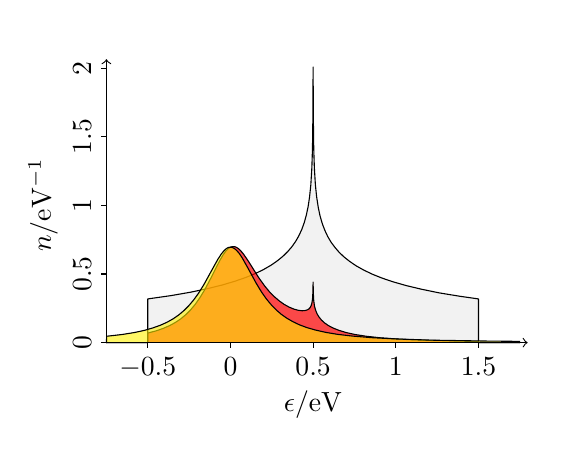
\begin{tikzpicture}[mark size=0.05cm, line cap=round]
	\draw [use as bounding box, draw=none]
		(-1.000, -1.000) rectangle +(6.750, 5.000);
	\draw [line join=round, fill opacity=0.05, fill=black] plot coordinates {
		(0.000, 0.000) (0.525, 0.000) (0.525, 0.555) (0.819, 0.597)
		(1.071, 0.641) (1.289, 0.687) (1.475, 0.733) (1.635, 0.781)
		(1.774, 0.829) (1.895, 0.879) (2.000, 0.931) (2.092, 0.984)
		(2.171, 1.039) (2.242, 1.097) (2.302, 1.156) (2.355, 1.217)
		(2.402, 1.284) (2.444, 1.357) (2.481, 1.437) (2.512, 1.523)
		(2.538, 1.616) (2.562, 1.729) (2.580, 1.850) (2.596, 2.004)
		(2.609, 2.218) (2.617, 2.463) (2.622, 2.851) (2.625, 3.500)
		(2.628, 2.851) (2.633, 2.463) (2.641, 2.218) (2.654, 2.004)
		(2.670, 1.850) (2.691, 1.714) (2.714, 1.606) (2.743, 1.507)
		(2.775, 1.424) (2.811, 1.347) (2.853, 1.276) (2.901, 1.211)
		(2.956, 1.147) (3.019, 1.087) (3.090, 1.031) (3.171, 0.976)
		(3.265, 0.923) (3.373, 0.871) (3.497, 0.821) (3.641, 0.772)
		(3.806, 0.725) (3.998, 0.679) (4.221, 0.633) (4.481, 0.590)
		(4.725, 0.555) (4.725, 0.000) (5.250, 0.000) };
	\draw [line join=round, fill opacity=0.7, fill=red] plot coordinates {
		(0.000, 0.000) (0.525, 0.000) (0.525, 0.122) (0.633, 0.150)
		(0.724, 0.182) (0.806, 0.218) (0.879, 0.258) (0.945, 0.303)
		(1.008, 0.355) (1.068, 0.415) (1.126, 0.484) (1.184, 0.566)
		(1.247, 0.669) (1.323, 0.813) (1.436, 1.036) (1.483, 1.117)
		(1.520, 1.167) (1.549, 1.195) (1.575, 1.212) (1.599, 1.220)
		(1.622, 1.220) (1.646, 1.213) (1.672, 1.197) (1.704, 1.169)
		(1.743, 1.122) (1.801, 1.037) (1.935, 0.824) (2.006, 0.725)
		(2.069, 0.648) (2.132, 0.584) (2.195, 0.530) (2.257, 0.486)
		(2.321, 0.451) (2.381, 0.426) (2.436, 0.411) (2.483, 0.405)
		(2.520, 0.407) (2.549, 0.415) (2.570, 0.427) (2.586, 0.444)
		(2.599, 0.467) (2.609, 0.500) (2.617, 0.548) (2.622, 0.629)
		(2.625, 0.768) (2.628, 0.623) (2.633, 0.534) (2.643, 0.461)
		(2.657, 0.412) (2.675, 0.367) (2.699, 0.327) (2.730, 0.288)
		(2.769, 0.252) (2.819, 0.217) (2.880, 0.185) (2.953, 0.156)
		(3.045, 0.128) (3.158, 0.103) (3.300, 0.081) (3.483, 0.061)
		(3.728, 0.044) (4.066, 0.029) (4.573, 0.018) (4.725, 0.015)
		(4.725, 0.000) (5.250, 0.000) };
	\draw [line join=round, fill opacity=0.6, fill=yellow] plot coordinates {
		(0.000, 0.000) (0.003, 0.081) (0.197, 0.103) (0.354, 0.128)
		(0.483, 0.156) (0.593, 0.188) (0.688, 0.222) (0.772, 0.260)
		(0.848, 0.303) (0.919, 0.352) (0.984, 0.407) (1.047, 0.470)
		(1.108, 0.542) (1.171, 0.629) (1.239, 0.739) (1.336, 0.916)
		(1.415, 1.058) (1.460, 1.127) (1.494, 1.168) (1.522, 1.194)
		(1.549, 1.208) (1.572, 1.212) (1.596, 1.209) (1.620, 1.199)
		(1.649, 1.176) (1.683, 1.138) (1.725, 1.076) (1.790, 0.960)
		(1.903, 0.753) (1.971, 0.641) (2.034, 0.552) (2.095, 0.479)
		(2.158, 0.414) (2.223, 0.358) (2.292, 0.310) (2.368, 0.266)
		(2.452, 0.226) (2.546, 0.191) (2.654, 0.160) (2.783, 0.131)
		(2.937, 0.105) (3.129, 0.083) (3.373, 0.063) (3.696, 0.046)
		(4.150, 0.031) (4.835, 0.020) (5.247, 0.016) (5.250, 0.000) };
	\draw [line cap=butt]
		(0.525, 0) -- +(0, -0.070) node [below] {$-0.5$}
		(1.575, 0) -- +(0, -0.070) node [below] {$0$}
		(2.625, 0) -- +(0, -0.070) node [below] {$0.5$}
		(3.675, 0) -- +(0, -0.070) node [below] {$1$}
		(4.725, 0) -- +(0, -0.070) node [below] {$1.5$}
		(0, 0.000) -- +(-0.070, 0) node [rotate=90, above] {$0$}
		(0, 0.872) -- +(-0.070, 0) node [rotate=90, above] {$0.5$}
		(0, 1.743) -- +(-0.070, 0) node [rotate=90, above] {$1$}
		(0, 2.615) -- +(-0.070, 0) node [rotate=90, above] {$1.5$}
		(0, 3.486) -- +(-0.070, 0) node [rotate=90, above] {$2$};
	\draw [<->, line cap=butt]
		(5.350, 0) -- (0, 0) -- (0, 3.600);
	\node [below=\baselineskip] at (2.625, -0.070)
		{$\epsilon / \mathrm{eV}$};
	\node [rotate=90, above=\baselineskip] at (-0.070, 1.750)
		{$n / \mathrm{eV^{-1}}$};
\end{tikzpicture}%

        \caption{$\omega = 0.2\,\mathrm{eV}$. At higher frequencies, exact and
                 approximate integrand may differ considerably.}
    \end{subfigure}%
    \hfill%
    \begin{subfigure}{6.75cm}
        % !TEX root = ../thesis.tex
%
\tikzsetnextfilename{const-dos-approx-2}
%
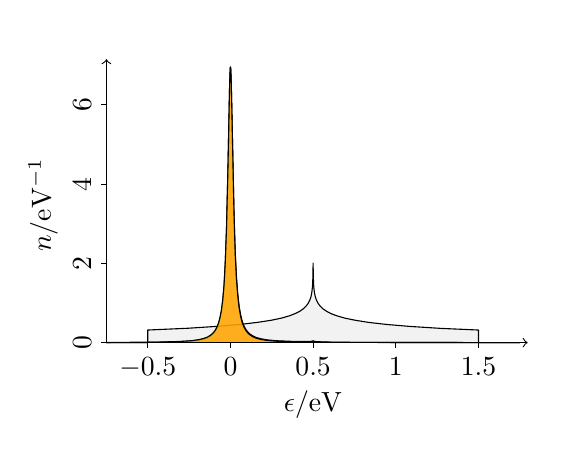
\begin{tikzpicture}[mark size=0.05cm, line cap=round]
	\draw [use as bounding box, draw=none]
		(-1.000, -1.000) rectangle +(6.750, 5.000);
	\draw [line join=round, fill opacity=0.05, fill=black] plot coordinates {
		(0.000, 0.000) (0.525, 0.000) (0.525, 0.160) (1.040, 0.183)
		(1.425, 0.208) (1.717, 0.233) (1.937, 0.260) (2.103, 0.286)
		(2.229, 0.313) (2.326, 0.341) (2.399, 0.370) (2.457, 0.399)
		(2.502, 0.431) (2.536, 0.464) (2.562, 0.499) (2.583, 0.540)
		(2.599, 0.588) (2.609, 0.640) (2.617, 0.711) (2.622, 0.823)
		(2.625, 1.010) (2.628, 0.823) (2.633, 0.711) (2.641, 0.640)
		(2.654, 0.579) (2.670, 0.534) (2.691, 0.495) (2.717, 0.461)
		(2.751, 0.429) (2.796, 0.398) (2.853, 0.368) (2.929, 0.340)
		(3.029, 0.311) (3.161, 0.284) (3.331, 0.257) (3.557, 0.231)
		(3.853, 0.206) (4.247, 0.181) (4.725, 0.160) (4.725, 0.000)
		(5.250, 0.000) };
	\draw [line join=round, fill opacity=0.7, fill=red] plot coordinates {
		(0.000, 0.000) (0.525, 0.000) (0.525, 0.004) (0.882, 0.010)
		(1.055, 0.019) (1.160, 0.031) (1.228, 0.045) (1.278, 0.062)
		(1.318, 0.083) (1.349, 0.108) (1.376, 0.138) (1.399, 0.177)
		(1.420, 0.226) (1.441, 0.298) (1.460, 0.391) (1.478, 0.531)
		(1.494, 0.714) (1.509, 0.992) (1.525, 1.424) (1.544, 2.213)
		(1.565, 3.281) (1.572, 3.483) (1.575, 3.500) (1.578, 3.490)
		(1.583, 3.392) (1.596, 2.824) (1.620, 1.674) (1.635, 1.170)
		(1.651, 0.842) (1.667, 0.628) (1.685, 0.464) (1.704, 0.356)
		(1.722, 0.281) (1.743, 0.221) (1.767, 0.174) (1.793, 0.138)
		(1.822, 0.110) (1.856, 0.087) (1.901, 0.066) (1.958, 0.050)
		(2.040, 0.035) (2.163, 0.024) (2.363, 0.016) (2.570, 0.015)
		(2.615, 0.018) (2.622, 0.021) (2.625, 0.026) (2.630, 0.019)
		(2.654, 0.014) (2.772, 0.008) (3.197, 0.003) (5.250, 0.000) };
	\draw [line join=round, fill opacity=0.6, fill=yellow] plot coordinates {
		(0.000, 0.000) (0.003, 0.002) (0.664, 0.007) (0.935, 0.015)
		(1.082, 0.025) (1.173, 0.038) (1.236, 0.053) (1.284, 0.071)
		(1.320, 0.093) (1.352, 0.120) (1.378, 0.152) (1.402, 0.194)
		(1.423, 0.248) (1.441, 0.314) (1.460, 0.409) (1.478, 0.551)
		(1.494, 0.736) (1.509, 1.017) (1.525, 1.452) (1.544, 2.240)
		(1.565, 3.294) (1.572, 3.486) (1.575, 3.500) (1.578, 3.486)
		(1.586, 3.294) (1.620, 1.644) (1.635, 1.141) (1.651, 0.817)
		(1.667, 0.605) (1.685, 0.444) (1.704, 0.337) (1.722, 0.264)
		(1.743, 0.206) (1.767, 0.160) (1.793, 0.125) (1.822, 0.099)
		(1.859, 0.075) (1.903, 0.056) (1.964, 0.040) (2.050, 0.027)
		(2.187, 0.016) (2.431, 0.008) (2.993, 0.003) (5.250, 0.000) };
	\draw [line cap=butt]
		(0.525, 0) -- +(0, -0.070) node [below] {$-0.5$}
		(1.575, 0) -- +(0, -0.070) node [below] {$0$}
		(2.625, 0) -- +(0, -0.070) node [below] {$0.5$}
		(3.675, 0) -- +(0, -0.070) node [below] {$1$}
		(4.725, 0) -- +(0, -0.070) node [below] {$1.5$}
		(0, 0.000) -- +(-0.070, 0) node [rotate=90, above] {$0$}
		(0, 1.006) -- +(-0.070, 0) node [rotate=90, above] {$2$}
		(0, 2.013) -- +(-0.070, 0) node [rotate=90, above] {$4$}
		(0, 3.019) -- +(-0.070, 0) node [rotate=90, above] {$6$};
	\draw [<->, line cap=butt]
		(5.350, 0) -- (0, 0) -- (0, 3.600);
	\node [below=\baselineskip] at (2.625, -0.070)
		{$\epsilon / \mathrm{eV}$};
	\node [rotate=90, above=\baselineskip] at (-0.070, 1.750)
		{$n / \mathrm{eV^{-1}}$};
\end{tikzpicture}%

        \caption{$\omega = 0.02\,\mathrm{eV}$. At lower frequencies, points for
                 numerical integration must be chosen carefully.}
    \end{subfigure}
    \captionsetup{singlelinecheck=off}
    \caption[Constant-DOS approximation]{ %
        The constant-DOS approximation is exemplified by its application to the
        scalar product of the density of states $n(\epsilon)$ of a square
        tight-binding lattice (compare Section $n$) and a \name{Lorentz}
        function:
        %
        \begin{align*}
            \int \from{-\infty} \till \infty
            \D \epsilon \, \frac {n(\epsilon)} \pi
            \frac \omega {\omega^2 + \epsilon^2}
            \quad
            (\tikz \draw [fill=red!70!white, rounded corners=3pt]
                (0, 0) rectangle (0.5, 0.2);)
            \quad \approx \quad
            \int \from{-\infty} \till \infty
            \D \epsilon \, \frac {n(0)} \pi
            \frac \omega {\omega^2 + \epsilon^2}.
            \quad
            (\tikz \draw [fill=yellow!60!white, rounded corners=3pt]
                (0, 0) rectangle (0.5, 0.2);)
        \end{align*}
        %
        The exact integral bears a close resemblance to those which occur in the
        local self energy (Eq.~\ref{local self-energy}).
        }
    \label{constant-DOS approximation}
\end{figure}

\subsection{\name{Coulomb} pseudo-potential}

\subsection{Real-axis equations}

In this section the analytic continuation of the self-energy or the
corresponding \name{Eliashberg} equations, which is complicated by the summation
over \name{Matsubara} frequencies, is performed within the constant-DOS
approximation.

The first step is to withdraw the dependence on \name{Matsubara} frequencies
from the \name{Green} function with the help of a spectral representation. Under
the energy integral,
%
\begin{equation*}
    \int \from{-\infty} \till \infty \D \epsilon \, \vec G_\epsilon(\I \omega_n)
    = -\frac 1 \pi
    \int \from{-\infty} \till \infty \D \omega' \,
    \frac 1 {\I \omega_n - \omega'}
    \Im \int \from{-\infty} \till \infty \D \epsilon \,
    \vec G_\epsilon(\omega'_+),
\end{equation*}
%
where $\omega'_+ = \omega' + \I 0^+$. The \name{Green} function matrix,
analytically continued to arbitrary frequency arguments $\omega$ and dependent
on energy $\epsilon_{\vec k}$ rather than wave number $\vec k$, reads
%
\begin{equation*}
    \vec G_\epsilon(\omega) = \frac
        { \omega Z(\omega) \vec \sigma_0
        + \phi(\omega) \vec \sigma_1
        + \epsilon \vec \sigma_3 }
        { \omega^2 Z^2(\omega)
        - \phi^2(\omega)
        - \epsilon^2}.
\end{equation*}
%
Using Eqs.~\ref{integrals} one finds, in accordance with Eq.~2.19a of
Ref.~\barecite{ScalapinoSchriefferWilkins66},
%
\begin{equation*}
    -\frac 1 \pi \int \from{-\infty} \till \infty \D \epsilon \,
    \vec G_\epsilon(\omega)
    = \frac
        {\omega Z(\omega) \vec \sigma_0 + \phi(\omega) \vec \sigma_1}
        {\sqrt{-\omega^2 Z^2(\omega) + \phi^2(\omega)}}
    = \I \frac
        {\omega Z(\omega) \vec \sigma_0 + \phi(\omega) \vec \sigma_1}
        {\sqrt[\dagger]{\omega^2 Z^2(\omega) - \phi^2(\omega)}}
    = \I \frac
        {\omega \vec \sigma_0 + \Delta(\omega) \vec \sigma_1}
        {\sqrt[*]{\omega^2 - \Delta^2(\omega)}}.
\end{equation*}
%
Let $\varphi$ represent the complex arguments of the above square roots. The
first square root is the principal one defined by $-\frac \pi 2 < \varphi \leq
\frac \pi 2$. Since a multiplication with $\I$ corresponds to a rotation by
$\frac \pi 2$ in the complex plane, the second square root must be taken from
the upper half-plane such that $0 < \varphi \leq \pi$
\cite[Eq.~2.19b]{ScalapinoSchriefferWilkins66}. Clockwise rotation by the
complex argument of $Z(\omega)$ yields the domain of the third square root for
which $-\arg[Z(\omega)] < \varphi \leq \pi - \arg[Z(\omega)]$.

Using $\Im[\I \dots] = \Re[\,\dots]$, the phononic part of the self-energy reads
%
\begin{multline*}
    \vec \Sigma \super{ph.} (\I \omega_n)
    = T \sum_m \int \from{-\infty} \till \infty \D \epsilon \,
    \vec \sigma_3 \, \vec G_\epsilon(\I \omega_m) \, \vec \sigma_3 \,
    \lambda(\I \omega_n - \I \omega_m)
    \\
    = T \int \from{-\infty} \till \infty \D \omega' \, \Re \bigg[ \frac
        {\omega'_+ \vec \sigma_0 - \Delta(\omega'_+) \vec \sigma_1}
        {\sqrt[*]{\omega'^2_+ - \Delta^2(\omega'_+)}}
    \bigg]
    \int \from 0 \till \infty \D \omega'' \, \alpha^2 F(\omega'')
    \sum_m \frac 1 {\I \omega_m - \omega'}
    \frac{2 \omega''}{(\omega_n - \omega_m)^2 + \omega''^2}.
\end{multline*}
%
It is now possible to eliminate the summation over \name{Matsubara} frequencies
\cite[Eqs.~3.40, 3.41]{AllenMitrovic82},
%
\begin{equation*}
    T \sum_m \frac 1 {\I \omega_m - \omega'}
    \frac{2 \omega''}{(\omega_n - \omega_m)^2 + \omega''^2}
    = \frac{f_+(-\omega') + f_-(\omega'')}{\I \omega_n - \omega' - \omega''}
    + \frac{f_+( \omega') + f_-(\omega'')}{\I \omega_n - \omega' + \omega''}
    \equiv \Omega(\I \omega_n, \omega', \omega''),
\end{equation*}
%
and to analytically continue the self-energy, which yields
%
\begin{equation*}
    \vec \Sigma \super{ph.} (\omega) =
    \int \from{-\infty} \till \infty \D \omega' \,
    \Re \bigg[ \frac
        {\omega'_+ \vec \sigma_0 - \Delta(\omega'_+) \vec \sigma_1}
        {\sqrt[*]{\omega'^2_+ - \Delta^2(\omega'_+)}}
    \bigg]
    \int \from 0 \till \infty \D \omega'' \, \alpha^2 F(\omega'') \,
    \Omega(\omega, \omega', \omega'').
\end{equation*}

With the identity \cite[Eq.~12.4]{AllenMitrovic82}
%
\begin{equation*}
    T \sum_m \frac 1 {\I \omega_n - \omega'} = -\frac 1 2 [1 - 2 f_+(\omega')]
\end{equation*}
%
the electronic part of the self-energy is analogously found to be
%
\begin{align*}
    \vec \Sigma \super{el.} (\omega)
    = \mu T \sum_{m} \int \from{-\infty} \till \infty \D \epsilon \,
    \vec G_{\vec q} \super{od.} (\omega)
    = -\frac \mu 2 \int \from{-\infty} \till \infty \D \omega' \,
    \Re \bigg[ \frac
        {\Delta(\omega'_+) \vec \sigma_1}
        {\sqrt[*]{\omega'^2_+ - \Delta^2(\omega'_+)}}
    \bigg] [1 - 2 f_+(\omega')].
\end{align*}

For $\vec \Sigma(\omega) = \vec \Sigma \super{ph.}(\omega) + \vec \Sigma
\super{el.}(\omega)$ the so-called \emph{real-axis Eliashberg equations}, which
are actually defined for the whole complex plane, are found to be
%
\begin{align*}
    Z(\omega) = 1 - \frac 1 \omega
    &\int \from{-\infty} \till \infty \D \omega' \,
    \Re \bigg[
        \frac{\omega'_+}{\sqrt[*]{\omega'^2_+ - \Delta^2(\omega'_+)}}
    \bigg] \int \from 0 \till \infty \D \omega'' \, \alpha^2 F(\omega'') \,
    \Omega(\omega, \omega', \omega''),
    \\
    \Delta(\omega) = -\frac 1 {Z(\omega)}
    &\int \from{-\infty} \till \infty \D \omega' \,
    \Re \bigg[
        \frac{\Delta(\omega'_+)}{\sqrt[*]{\omega'^2_+ - \Delta^2(\omega'_+)}}
    \bigg]
    \bigg \{
        [1 - 2 f_+(\omega')] \, \frac \mu 2
        + \int \from 0 \till \infty \D \omega'' \, \alpha^2 F(\omega'') \,
        \Omega(\omega, \omega', \omega'')
    \bigg \}.
\end{align*}

Let $f(\omega)$ represent any of the functions $\omega^2$, $Z(\omega)$ and
$\phi(\omega)$. They all have in common that they transform into their complex
conjugate if the sign of either the real or imaginary part of their argument
changes \cite[Eq.~A5]{AmbegaokarTewordt64}. Formally,
%
\begin{equation*}
    f(-\omega) = f(\omega) \quad \text{and} \quad f(\omega^*) = f^*(\omega).
\end{equation*}
%
The same applies to functions which are derived by means of the four basic
arithmetical operations, such as $\Delta(\omega) = \phi(\omega) / Z(\omega)$,
$\omega^2 + \Delta^2(\omega)$ or $\omega^2 Z^2(\omega) + \phi^2(\omega)$.
Complex conjugation reflects a number across the real axis and its square roots
across any of the axes which span the complex plane, i.e. from odd- to
even-numbered quadrants or vice versa if the number is not real. As a
consequence, sign changes of $\Im[\omega^2 + \Delta^2(\omega)]$ and
$\Re[\sqrt[*]{\omega^2 + \Delta^2(\omega)}]$ are coupled. Note that the domain
of $\sqrt[*] \cdots$ changes with $Z(\omega)$.

These symmetries are now used to fold the negative half of the range of the
$\omega'$ integral onto the positive one, which yields the final form of the
real-axis \name{Eliashberg} equations:
%
\begin{subequations} \label{real-axis Eliashberg equations}
    \begin{align} \notag
        Z(\omega) = 1 - \frac 1 \omega
        &\int \from 0 \till \infty \D \omega' \,
        \Re \bigg[
            \frac{\omega'_+}{\sqrt[*]{\omega'^2_+ - \Delta^2(\omega'_+)}}
        \bigg]
        \times \dots
        \\ \label{Z(omega)}
        \dots \times
        &\int \from 0 \till \infty \D \omega'' \, \alpha^2 F(\omega'') \,
        [ \Omega(\omega,  \omega', \omega'')
        + \Omega(\omega, -\omega', \omega'') ],
        \\ \notag
        \Delta(\omega) = -\frac 1 {Z(\omega)}
        &\int \from 0 \till \infty \D \omega' \,
        \Re \bigg[ \frac
            {\Delta(\omega'_+)}
            {\sqrt[*]{\omega'^2_+ - \Delta^2(\omega'_+)}}
        \bigg]
        \bigg \{
            [1 - 2 f_+(\omega')] \, \mu
            + \dots
            \\
            \dots +
            &\int \from 0 \till \infty \D \omega'' \, \alpha^2 F(\omega'') \,
            [ \Omega(\omega,  \omega', \omega'')
            - \Omega(\omega, -\omega', \omega'') ]
        \bigg \}.
    \end{align}
\end{subequations}
%
The $\omega$ in the denominator of Eq.~\ref{Z(omega)} is cancelled since, where
braces enclose alternatives,
%
\begin{equation*}
    \frac {
        \Omega(\omega,  \omega', \omega'') \pm
        \Omega(\omega, -\omega', \omega'')
        } 2
    = \begin{Bmatrix} \omega \\ \omega' + \omega'' \end{Bmatrix}
    \frac
        {f_+(-\omega') + f_-(\omega'')}
        {\omega^2 -(\omega' + \omega'')^2}
    + \begin{Bmatrix} \omega \\ \omega' - \omega'' \end{Bmatrix}
    \frac
        {f_+(\omega') + f_-(\omega'')}
        {\omega^2 -(\omega' - \omega'')^2}.
\end{equation*}

\section{\name{McMillan}'s formula}

In 1968, William L. \name{McMillan} established a formula to estimate the
transition temperature $T \sub c$ of the superconducting state from only three
characteristic parameters: an average phonon frequency $\av \omega$, the
electron-phonon coupling strength $\lambda$ and the \name{Coulomb}
pseudo-potential $\mu^*$. This section provides a review of the original work
\cite{McMillan68}.

The starting point is a linearized form of the real-axis \name{Eliashberg}
equations. At $T \sub c$, the order parameter $\Delta(\omega)$ is infinitesimal
and can be neglected relative to $\omega$. Introducing two cutoff energies, the
maximum phonon frequency $\omega_0$ and the electronic bandwidth $E \sub B$,
Eq.~\ref{real-axis Eliashberg equations} becomes
%
\begin{align*}
    Z(\omega) = 1 - \frac 1 \omega
    \int \from 0 \till \infty \D \omega'
    &\int \from 0 \till{\omega_0} \D \omega'' \, \alpha^2 F(\omega'') \,
    [\Omega(\omega, \omega', \omega'') + \Omega(\omega, -\omega', \omega'')],
    \\
    \Delta(\omega) = -\frac 1 {Z(\omega)}
    \int \from 0 \till \infty \D \omega' \,
    \!&\,\frac{\Re[\Delta(\omega')]}{\omega'}
    \Big \{
        \Theta(E \sub B - \omega') \, [1 - 2 f_+(\omega')] \, \mu
        + \dots
        \\
        \dots +
        &\int \from 0 \till{\omega_0} \D \omega'' \, \alpha^2 F(\omega'') \,
        [\Omega(\omega, \omega', \omega'') - \Omega(\omega, -\omega', \omega'')]
    \Big \}.
\end{align*}

The idea is to find an analytical expression which roughly approximates $T \sub
c$ and can be used to fit numerical results. To that end, a simple trial
function for $\Delta(\omega)$ is introduced, which shall solve the
\name{Eliashberg} equations, i.e. be self-consistent, at least at low and high
frequencies:
%
\begin{equation*}
    \Delta(\omega) = \begin{cases}
        \Delta_0 & \text{for $|\omega| < \omega_0$,} \\
        \Delta_\infty & \text{otherwise,}
    \end{cases}
\end{equation*}
%
where $\Delta_0, \Delta_\infty \in \mathds R$. Several approximate contributions
to $\Delta(0)$ and $\Delta(\infty)$ are taken into account:
%
\begin{enumerate}
    \item \textbf{Phononic contribution to \bm$\Delta(0)$ for \bm$\omega' <
    \omega_0$.} Neglecting $\omega'$ relative to $\omega''$ yields
    %
    \begin{gather*}
        \Omega(0, \omega', \omega'') - \Omega(0, -\omega', \omega'')
        \approx -\frac 2 {\omega''} [1 - 2 f_+(\omega')],
        \\
        \Delta^{(1)}(0) \approx \frac{\Delta_0}{Z(0)}
        \hypo
            {\int_0^{\omega_0} \frac{\D \omega'}{\omega'}
            \hyper{[1 - 2 f_+(\omega')]}{\approx \Theta(\omega' - T \sub c)}}
            {\approx \ln(\omega_0 / T \sub c)} \
        \hypo
            {2 \int_0^{\omega_0} \frac{\D \omega''}{\omega''}
            \alpha^2 F(\omega'')}{\equiv \lambda},
    \end{gather*}
    %
    where the \emph{electron-phonon coupling strength} $\lambda$ has been
    defined.
    %
    \item \textbf{Phononic contribution to \bm$\Delta(0)$ for \bm$\omega' \geq
    \omega_0$.} Neglecting $\omega''$ relative to $\omega'$ yields
    %
    \begin{gather*}
        \Omega(0, \omega', \omega'') - \Omega(0, -\omega', \omega'')
        \approx -\frac 2 {\omega'} [1 - 2 f_-(\omega'')],
        \\
        \Delta^{(2)}(0) \approx \frac{\Delta_\infty \lambda}{Z(0)}
        \hypo
            {\int_{\omega_0}^\infty \frac{\D \omega'}{\omega'^2}}
            {= 1 / \omega_0} \
        \hypo
            {\frac 2 \lambda \int \from 0 \till{\omega_0} \D \omega'' \,
            \alpha^2 F(\omega'')}{\equiv \av \omega}
        \hypo{[1 - 2 f_-(\omega'')]}{\approx 1},
    \end{gather*}
    %
    where an \emph{average phonon frequency} $\av \omega$ has been defined.
    %
    \item \textbf{Phononic contribution to \bm$\Delta(\infty)$.} This part
    vanishes for $\Omega(\infty, \omega', \omega'') - \Omega(\infty, -\omega',
    \omega'') = 0$.
    %
    \item \textbf{Electronic contribution to \bm$\Delta(0)$.} Approximating the
    distributions as in $\Delta^{(1)}(0)$ and $\Delta^{(2)}(0)$,
    %
    \begin{equation*}
        \Delta^{(3)}(0) = -\frac \mu {Z(0)} \bigg[
            \Delta_0 \hypo
                {\int_0^{\omega_0} \frac{\D \omega'}{\omega'}
                \hyper
                    {[1 - 2 f_+(\omega')]}
                    {\approx \Theta(\omega' - T \sub c)}}
                {\approx \ln(\omega_0 / T \sub c)}
            + \Delta_\infty \hypo
                {\int_{\omega_0}^{E \sub B}
                \frac{\D \omega'}{\omega'}}{= \ln(E \sub B / \omega_0)}
            \hypo{[1 - 2 f_+(\omega')]}{\approx 1}
        \bigg].
    \end{equation*}
    %
    \item \textbf{Electronic contribution to \bm$\Delta(\infty)$.} Analogous to
    the calculation of $\Delta^{(3)}(0)$,
    %
    \begin{equation*}
        \Delta(\infty) \approx -\frac \mu {Z(\infty)} \bigg[
            \Delta_0 \ln \frac{\omega_0}{T \sub c}
            + \Delta_\infty \ln \frac{E \sub B}{\omega_0}
        \bigg].
    \end{equation*}
\end{enumerate}

\section{Computational implementation}
